\subsection{EMG-forstærker}

EMG-forstærkeren testes for at vurdere, hvorvidt der kan opsamles muskelaktivitet fra rectus femoris. Overfladeelektroderne placeres ud fra SENIAM's anvisning om elektrodeplacering, jf. \autoref{sec:pilotforsoeg}. En squat-øvelse udføres, mens muskelsignaler opsamles i MATLAB. Denne øvelse er beskrevet i \autoref{sec:knaeled_squat}. Muskelsignalet under udførslen af squat-øvelsen fremgår af \autoref{fig:raat_emg}. 

\begin{figure}[H]
\centering
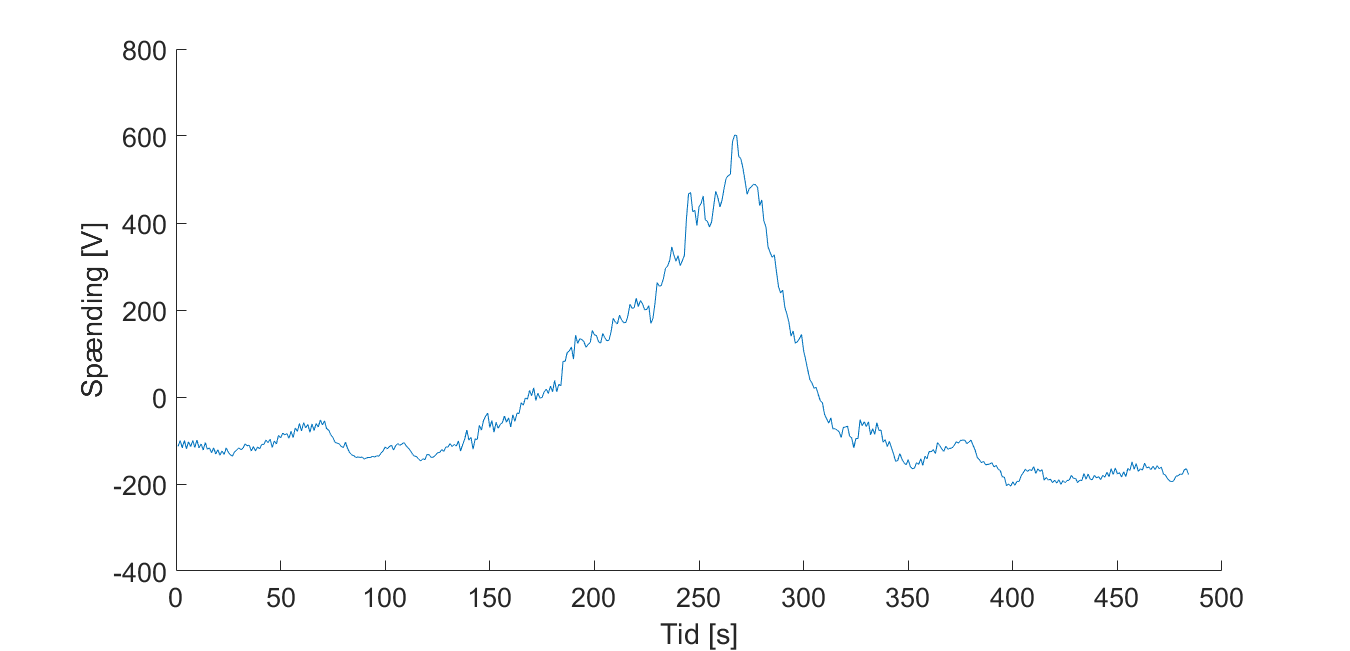
\includegraphics[width=0.9\textwidth]{figures/raat_EMG_test}
\caption{Et samplede EMG-signal fra rectus femoris under udførsel af en squat-øvelse.}
\label{fig:raat_emg}
\end{figure}

\noindent
På EMG-forstærkeren findes et justerbart gain, således forstærkningen kan tilpasses den enkelte bruger af systemet. Ud fra dette og \autoref{fig:raat_emg} vurderes det, at EMG-forstærkeren opfylder de opstillede krav i \autoref{sec:EMG_krav}.

\textbf{Opsummering af krav:}
\begin{itemize}
\item[\Checkmark] Skal opsamle signaler fra rectus femoris
\item[\Checkmark] Skal være anvendeligt med overflade elektroder
\item[\Checkmark] Skal opsamle muskelsignaler i frekvensområdet mellem $10-500~Hz$
\item[\Checkmark] Skal forsynes med en spænding på minimum $\pm5~V$
\item[\Checkmark] Skal have et justerbart gain, der ikke kan forstærke over ADC'ens arbejdsområde
\end{itemize}


\subsection{Accelerometre}

Accelerometrene testes for at vurdere, hvorvidt de opstillede krav i \autoref{sec:acc_teori} opfyldes. Der tages udgangspunkt i værdierne fra databladet for ADXL335 \citep{analogdevices2010}, da det ikke er muligt at teste alle opstillede krav. Databladet oplyser, at de kan forsynes med en DC-forsyning fra $1,8-3,6~V$. Da accelerometrene skal kunne forsynes med en spænding på $3,3~V$, opfyldes dette krav. Herudover ses det ud fra databladet, at der er en linearitet med en afvigelse på $0,3\%$ samt et lineært arbejdsområde på $ \pm 3 g$. Af databladet fremgår det ligeledes, at accelerometrene er triaksiale. Det er derfor muligt at måle på minimum én akse, hvilket er det opstillede krav. Af denne grund er opfylder accelerometrene kravene.  

